\section{Intel 486}

\begin{wrapfigure}[5]{r}{0.25\textwidth}
\centering
\includegraphics[width=.25\textwidth]{drawings/intel_logo.pdf}
\end{wrapfigure}

486(80486)在 1989 年发布,是 80386 的一次性能演进,解决了 80386 的所有瓶颈。然而它 950 美元(2018 年约 1,920 美元)的售价让多数消费者望而却步。到 1993 年它终于变得可负担(500 美元),并成为 \doom{} 推荐的 CPU。\\
\par
与前代相比,设计变化很大。流水线增加了两个阶段,深度扩展到五级。此前可选且位于主板某处的 FPU\footnote{Floating Point Unit.} 被集成到芯片内部。最重要的是,制造工艺的改进\footnote{1.0$\mu$ 工艺(对比 i386 的 1.5$\mu$)以及晶圆面积增大,使得晶体管数量提升五倍,达到 120 万(i386 为 27.5 万)。它是首个晶体管数量超过一百万的 x86 芯片。} 让 486 能采用更复杂的设计,终于集成了 L1 缓存——这是 Intel 在 386 上尝试但失败的功能。\\
\par
\fq{386 实际上有一个很小的缓存,但最终被取消了,因为在我们能放到芯片上的缓存大小下,它性能不够。问题在于如果做更大的芯片,它会大到无法放进光刻机的视场去把图案曝光到芯片上。}{Gene Hill - Intel 386 Microprocessor Design and Development}\\
\par
{
\setlength{\belowcaptionskip}{-10pt}
\drawing{486_arch}{Intel 486 架构。}
}
\pagebreak
和 386 类似,Intel 以两种型号营销新 CPU。DX 是完整技术版本,而 SX 缺少 FPU。坊间流传一个经久不衰的神话:DX/SX 区分是 Intel 的营销把戏,用来卖出制造缺陷的芯片。实际上这是一个有意的商业策略\footnote{来源:“Lies, Damn Lies, and Wikipedia” by Michal Necasek;该时间线并不合理,因为“486DX 在 1989 年末开始量产,而 486SX 直到 1991 年中才发布。在最初 18 个月里良率问题最严重时,根本没有 SX。”。},以提供 50\% 的折扣价和销售 i487 FPU 协处理器的机会。\footnote{有趣的是,i487 FPU 升级实际上是一颗完整的 486DX,并会彻底禁用 486SX。}\\
\par
回顾来看,486 是 Intel 在 1994 年的冠军且无可争议的强者(性能与销量皆然\footnote{截至 2015 年末,486 仍被生产并用于网络路由器内。}),但它也经历过一段不确定时期。就像 386 要面对兄弟 i960 一样,i486 也要面对同厂的挑战者“Intel 860”。\\
\par
\fq{

\begin{wrapfigure}[11]{r}{0.55\textwidth}
\centering
\scaledimage{0.55}{i860.png}
\end{wrapfigure}

……我们在几乎同一时间推出了两颗非常强大的芯片:基于 CISC 技术、与所有 PC 软件兼容的 486;以及基于 RISC 技术、速度很快但与任何软件都不兼容的 i860。我们不知道该怎么做,于是两颗都推出,让市场决定。然而事情并不简单。支持一套微处理器架构所需的所有计算机相关产品——软件、销售、技术支持——需要巨大的资源。即便是 Intel,也只能勉强把一套架构做好。而我们现在有两套不同且相互竞争的架构,每一套都在不断消耗更多内部资源。研发项目往往像芥菜种子一样膨胀。为争夺资源和营销注意力(比如见客户时该重点推哪颗处理器)而爆发的内部争论,激烈到足以撕裂我们的微处理器组织。与此同时,我们的摇摆也让客户疑惑 Intel 到底代表什么:486 还是 i860?}{Andy Grove, “Only the paranoid survive”}





在纸面上,i860 很惊艳,是个严肃的对手。它采用重度流水线的超标量架构并压榨 VLIW\footnote{Very Long Instruction Word.},有 X、Y、Z 三个单元允许并行处理,若高效使用可超越 Intel 486。\\
\par
但与后来的 Pentium 等 CPU 通过自动并行执行指令来隐藏芯片复杂性不同,i860 的架构要求直接操控其并行流水线。芯片本身不做任何“幕后”工作,完全依赖编译器作者来安排指令序列。\\
\par
可惜当时编译器技术还不成熟。在缺乏 Intel 全力支持来打造关键工具的情况下,现有编译器完全无法生成能发挥其超标量能力的指令。i860 从未能发挥全部潜力。若 Intel 当时愿意打造所需工具,i860 的历史可能会截然不同。\\
\par
\par
\cscaledimage{0.85}{i486DX.png}{Intel 80486 封装。}
\par
图 \ref{i486DX.png} 展示了 Intel 486 的裸片,包含 1,180,235 个晶体管。大约在这个时期,Intel 开始在 CPU 上印上注册商标的标志,以与日益激进的 AMD 与 Cyrix 兼容芯片拉开距离。\\
\par
\trivia{i860 与 \doom{} 也有一点联系,因为它被用于 NeXTDimension 的视频处理板。}

\par
\subsection{流水线改进}
将 486 的 MIPS 性能与上一代进行对比,性能提升非常直观。得益于更好的制造工艺,顶级 486 可达到 50MHz\footnote{达到该频率的 486 DX 50MHz 采用 1.0$\mu$ 工艺制造。},但频率提升并非改进的主要来源。\\
\par
仔细观察图表可以发现,即便在相同频率下,486 的处理能力也超过 386 的两倍。\\

\par
\begin{figure}[H]
\centering
  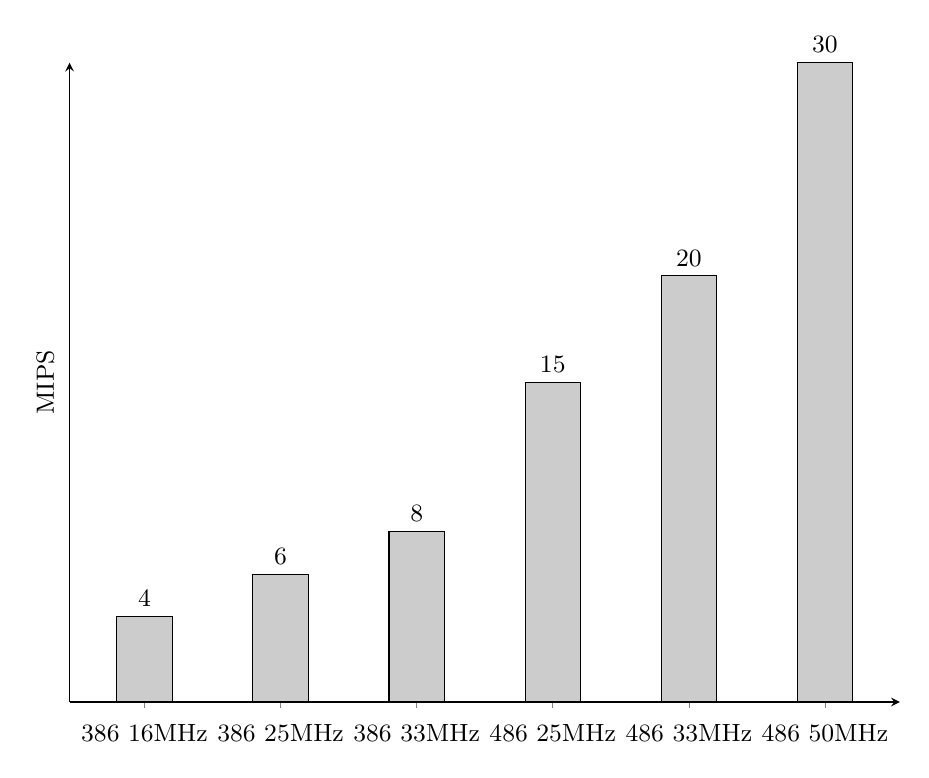
\begin{tikzpicture}[font=\small]
    \begin{axis}[
      width=1.0\textwidth,
      height=0.8\textwidth,
      ybar,
      bar width=20pt,
      ylabel={MIPS},
      ymin=0,
      ytick=\empty,
      xtick=data,
      axis x line=bottom,
      axis y line=left,
      enlarge x limits=0.11,
      symbolic x coords={386 16MHz,386 25MHz,386 33MHz,486 25MHz,486 33MHz,486 50MHz},
      xticklabel style={anchor=base,yshift=-\baselineskip},
      nodes near coords={\pgfmathprintnumber\pgfplotspointmeta}
    ]
      \addplot[fill=black!20,draw=black] coordinates {
        (386 16MHz,4)
        (386 25MHz,6)
        (386 33MHz,8)
        (486 25MHz,15)
        (486 33MHz,20)
        (486 50MHz,30)
      };
    \end{axis}
   
   \end{tikzpicture}
   \caption{Intel CPU 的 MIPS 对比\protect\footnotemark。}
 \end{figure}
\footnotetext{“每秒百万指令(MIPS)”。来源:Roy Longbottom 的 PC Benchmark:http://www.roylongbottom.org.uk/mips.htm。}

其性能提升来自更高的平均吞吐量。官方文档将 386 描述为三级流水线处理器。图 \ref{386_doc_pipeline} 显示在理想条件下,它应该能做到每个周期执行一条指令。实际中 CPU 的行为如图 \ref{386_real_pipeline},比文档建议慢了两倍。

\begin{figure}[H]
\centering
\includegraphics[width=\textwidth]{drawings/386_instruction_pipeline.pdf}
\caption{根据 Intel 文档的 386 理论流水线。}
\label{386_doc_pipeline}
\end{figure}



\par
即使预取单元和执行单元得到充分供给,解码单元解码一条指令也至少需要两个周期\footnote{解码很复杂,因为 x86 使用变长指令,而不是 RISC 的定长方式。}。由于流水线的最大吞吐量受最慢阶段限制,Intel 386 最多只能每两周期处理一条指令。\\
\par

\begin{figure}[H]
\centering
\includegraphics[width=\textwidth]{drawings/actual_386_instruction_pipeline.pdf}
\caption{实际中的 386 流水线:每条指令两周期。}
\label{386_real_pipeline}
\end{figure}

\par
为解决该问题,Intel 将三段流水线拆成五段(预取、解码1、解码2、执行、回写)。在各阶段都保持 1 CPI\footnote{Cycle Per Instruction。} 的情况下,486 的总吞吐量翻倍(只要流水线不被饿死)。\\
\par
\begin{figure}[H]
\centering
\includegraphics[width=\textwidth]{drawings/actual_486_instruction_pipeline.pdf}
\caption{486 流水线:每条指令一周期。}
\end{figure}
\par



\par





\subsection{缓存}
改进流水线并让各阶段运行速度一致,是向前迈出的一步。但更深的流水线也更容易饿死。从空流水线开始,486 的延迟为 5 个周期,而 386 是 4 个周期。若 486 经常停顿,它会比 386 还慢。由于缺失数据或指令而导致的停顿必须被尽可能避免。\\
\par
从技术角度看,这似乎是个难题。自 1980 年以来,RAM 性能一直落后于 CPU 性能。每年 CPU 性能提升 60\%,而 DRAM 仅提升 7\%,差距每年扩大 50\%。到 1989 年,DRAM 访问时间已比 CPU 周期时间慢 10 倍。\\
\par
\vspace{2mm}
\drawing{ram_vs_cpu}{来源:“Computer Organization and Design” by Hennessy and Patterson}
\par
在 486 之前,CPU 从 DRAM 请求指令或数据时必须停顿,通过总线单元与主板内存控制器通信。尽管 ISA 总线协议已相当优化,也至少需要两个周期。\\
\par 
第一周期初始化总线请求,在地址线上放置地址并设置控制线(读/写)。然后进入等待周期(Intel 称为 Wait State,因为等待总线单元时 CPU 什么都不做),由总线另一端的设备完成请求。\\
\par
\drawing{cpu_chipset_bus}{386 的 CPU-RAM 通信元素。}
\par
如果设备能在首个等待周期内响应,总线请求可在零等待状态完成,CPU 继续执行。否则会插入额外 Wait State 直到请求完成。从性能角度看,这些 Wait State 是灾难性的,不仅让指令耗时更长,还会阻塞流水线中的所有其它指令。\\
\par
\rawdrawing{cpu_wait_states}
\par
两周期的总线请求是 CPU 所能达到的最快速度。实际中 DRAM 访问往往需要插入多个 Wait State。
要避免这一点,就意味着完全避免使用总线。因此,Intel 在流水线与总线单元之间加入了一个新组件:L1(一级)缓存。其思路是利用程序的时间局部性与空间局部性。\\
\par
时间局部性来源于程序的迭代特性。处于循环时,刚访问过的指令在下一次迭代中很可能再次被访问。空间局部性与程序顺序读写数据数组有关:当访问一个内存地址时,邻近地址很可能也会在不久后被访问。\\
\par
利用这两种特性,设计良好的缓存放在 CPU 与总线单元之间时,经常已经包含了所需数据或指令,从而无需总线请求。\\
\par
\drawing{cpu_cache}{486 的 CPU-RAM 通信元素。}



\vspace{-20pt}
\subsection{L1 缓存}
希望到这里已经很清楚,缓存是整个 CPU 的基石。设计缓存以获得尽可能高的命中率,并让它尽可能快,是至关重要的。

\subsubsection{DRAM vs SRAM}
缓存的第一个优势是更低的 RAM 延迟。SIMM 插槽中的主内存使用 DRAM(动态 RAM),而缓存使用另一种称为 SRAM(静态 RAM)的类型,访问速度更快。DRAM 的典型访问时间为 200ns,而 SRAM 可达到 20ns,快 10 倍。\\
\par
速度差异来自其基本存储单元的设计。\\
\par
DRAM 单元存储 1 bit。其设计简单,包含一个晶体管和一个存储电容,能够高密度堆叠、容量大。但电容会随时间及每次访问而放电。每次读取后必须写回其值,即使不访问也需要每 15$\mu s$ 刷新一次。\\
\par
\scaleddrawing{1}{DRAM}{动态 RAM 及其存储 1 bit 数据的两个元件。}
\vspace{-5pt}
DRAM 的缓慢来自每个单元的高维护成本。它还有距离上的劣势:位于主板某处,需要使用与其他设备共享的 ISA 总线。\\
\par

\vspace{2mm}
得益于更复杂的设计(密度更低、制造更贵),SRAM 单元没有这些缺点。\\
\par
\scaleddrawing{1}{SRAM}{由六个元件构成的静态 RAM。}
\par
没有电容的 SRAM 单元不会漏电,不需要周期刷新,也不需要每次访问后写回。其两根位线能实现更快的电压变化检测与更快的时序。
由于它位于 CPU 芯片内部,访问不需要昂贵的总线请求,也不会与其他设备争用\footnote{DRAM 速度随后有所改善。Fast Page Mode 会用 SDRAM 行缓冲“缓存”DRAM 的行。udacity.com 的 UPCF 课程若想深入了解该主题很值得一看。}。
\par








\subsubsection{缓存行}
L1 缓存不仅硬件更好,设计也很巧妙。它体积小(8 KiB)且负载重(代码与数据统一缓存),但仍在正常工作时达到了令人印象深刻的 92\% 命中率\footnote{来源:“The i486 CPU: Executing Instructions in One Clock Cycle”。}。\\
\par
为达成这一点,Intel 工程师采用了四路组相联设计,将 $2^{32}$ 地址空间分成 2,097,152 个 2 KiB 页面。每个页面内有 128 行 16 字节的缓存行(cacheline)。\\
\par
\drawing{cacheline}{缓存行中的 16 字节。}
\par
缓存系统由一个目录和四个 bank(也称为 way)组成。每个 way 可存储 128 条 16 字节的缓存行,因此容量为 2 KiB。这些 16 字节的行就是缓存的基本单位。\\
\drawing{mem_to_way}{缓存控制器如何解析内存地址。}
\par
当接收到 32 位地址访问请求时,缓存控制器将其拆分为图 \ref{mem_to_way} 所示的三段,并执行以下步骤。
\begin{enumerate}
\item 使用 LINE 字段 [4-10] 查找 128 条目录项之一。
\item 查看该目录项中的四个 tag。若有一个与 TAG [11-31] 匹配,则表示该缓存行存在于四个 way 之一。
\item 检查目录项中的标志 F,确认该缓存行有效。
\item 使用 OFFSET [0-3] 字段访问缓存行中的 16 个值之一。
\item 更新目录项中的标志 F,以更新 LRU\footnote{Least Recently Used。} 值。
\end{enumerate}
\par
某个内存地址的内容可以位于四个 way 中的任意一个,但总是在相同的 LINE 偏移处。由于 $2^{32} / 128 = 33,554,432$ 个地址争夺 4 个槽位,缓存行的逐出不可避免,并通过 LRU 策略仲裁\footnote{逐出既可能发生在读操作中,也可能发生在写操作中,如果缓存为写分配模式,而所有 Intel 486 都是写分配(来源:“Internal Cache Architecture of X86 Processors”)。}。\\
\par
\drawing{cacheways}{缓存控制器与四个 way(bank)。}
\par
\trivia{为什么不增加 way 数或缓存大小?在 8 KiB 缓存下,四路提供了最佳折衷\footnote{来源:“Computer Architecture: A Quantitative Approach” by Hennessy/Patterson。}。两路缓存的未命中率为 14\%,四路为 10.5\%,但增加到八路仅提升到 10\%,全相联也只是 9\%。}\\
\par

\rawscaleddrawing{0.9}{set_state_caches}



\subsection{总线突发传输}
486 流水线中的任何缓存未命中都会触发缓存行逐出,并需要将整整 16 字节从 DRAM 传入 SRAM\footnote{预取器也以 16 字节为单位工作。它会取回并将缓存行存入 32 字节的预取队列。}。通常这会是非常昂贵的操作,也是 CPU 的重大问题。但 Intel 加入了所谓“突发传输(Burst Transfer)”能力来配合。\\
\par
原理很简单:在等待数据到达时,预先锁存下一次请求,这样总线控制器可以直接使用它,而无需等待 CPU 初始化新的总线请求。\\
\par
\drawing{netburst}{“突发传输”使缓存行填充速度提升 65\%。}






\subsection{Overdrive 与 L1 写回}
Intel 通过 80486 OverDrive 系列芯片将性能提高了 33\%。这些 CPU 具有倍频器,使其运行频率是总线的两倍(33MHz 型号 CPU 以 66MHz 运行)\footnote{直到今天,设计者仍在努力解决 CPU 远快于总线的难题。}。此外,L1 缓存策略改为写回(write-back,而非 write-through),显著降低了总线流量。\\
\par 
\vspace{10pt}
\scaleddrawing{0.9}{486dx2_notm}{“DX2-66” 是当时运行 \doom{} 的黄金标准}%{Best CPU to run \doom at the time.}
\par
%\trivia{Want even more performance? Not only a DX2-66 ran faster, they also came with an enhanced writeback L1 cache\footnote{The standard 486 L1 cache was writethrough with post-writes.}}

\begin{figure}[H]
\centering
  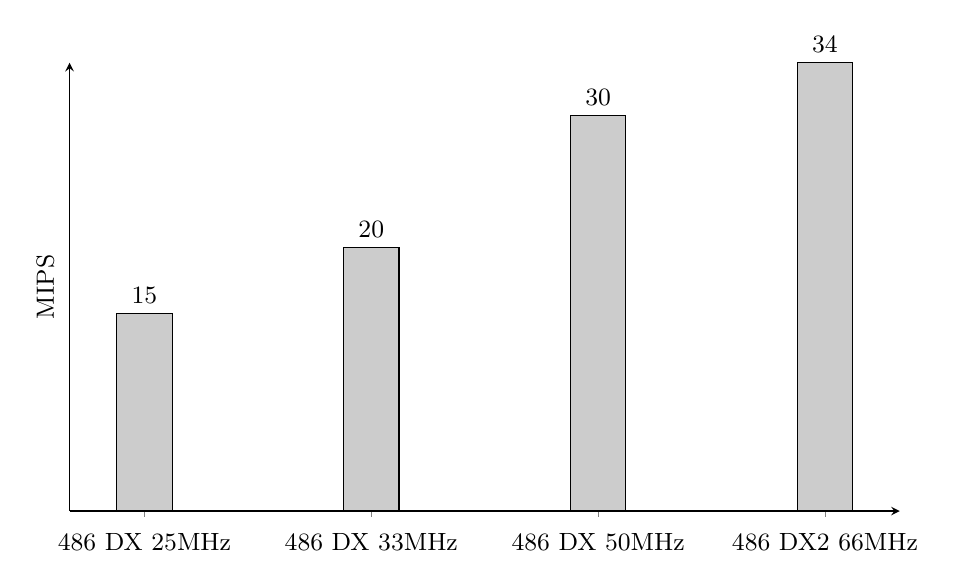
\begin{tikzpicture}[font=\small]
    \begin{axis}[
      width=1.0\textwidth,
      height=0.6\textwidth,
      ybar,
      bar width=20pt,
      ylabel={MIPS},
      ymin=0,
      ytick=\empty,
      xtick=data,
      axis x line=bottom,
      axis y line=left,
      enlarge x limits=0.11,
      symbolic x coords={486 DX 25MHz,486 DX 33MHz,486 DX 50MHz,486 DX2 66MHz},
      xticklabel style={anchor=base,yshift=-\baselineskip},
      nodes near coords={\pgfmathprintnumber\pgfplotspointmeta}
    ]
      \addplot[fill=black!20,draw=black] coordinates {
        (486 DX 25MHz,15)
        (486 DX 33MHz,20)
        (486 DX 50MHz,30)
        (486 DX2 66MHz,34)
      };
    \end{axis}
   
   \end{tikzpicture}
   \caption{CPU 的 MIPS 对比\protect\footnotemark。}
 \end{figure}
\footnotetext{来源:“Roy Longbottom's PC Benchmark Collection: http://www.roylongbottom.org.uk/mips.htm”。}
\par
观察上图可见,486DX2-66MHz 的速度快于 486DX-50MHz,但没有频率差异所暗示的 20\% 全幅提升。这是因为 DX2 的总线运行在 33MHz,而 DX 的 CPU 与总线都在 50MHz。




\subsection{裸片}
%To close this section on the 486, I cannot resist including a magnified photography of the die. 
如果你手中有本书的实体 9.25''x7.5'' 版本,CPU 封装为 30mm 正方形,裸片为 15.5 x 9.9 mm,均按 1:1 比例呈现。\\
\par
\bigskip

  \begin{figure}[!htb]

\begin{minipage}{0.48\textwidth}
\centering
\scaledrawimage{44.45mm}{486topdown.png}
%\caption{468 packaging.}
\end{minipage}
\hfill
\begin{minipage}{0.48\textwidth}
\centering
\includegraphics[width=44.45mm]{drawings/486toscale.pdf}
%\caption{The die inside the package.}
\end{minipage}
\end{figure}

\par



\begin{figure}[H]
\centering
\scaledimage{0.9}{486_blueprint.png}
\end{figure}
\par
\begin{figure}[H]
\centering
\scaledimage{0.9}{486_layout.png}
\end{figure}





\trivia{上一页中,数据通路与控制通路的晶体管布局不同:数据通路是手工设计的,控制通路则使用专为 486 打造的 CAD 工具生成\footnote{来源:Coping with the Complexity of Microprocessor Design at Intel -- A CAD History。}。}\\
\par
\subsection{为 486 编程}
有了架构背景,我们就能理解程序员如何充分利用 486。好消息是,性能提升的大部分是 90 年代“白捡”的免费午餐。同样的二进制在新 CPU 上会快两倍。\\
\par
除了少数特性\footnote{“Pushing the 486” by Michael Abrash。}之外,只要程序员注意缓存行并最大化时间与空间局部性\footnote{并避免分支。由于没有分支预测器,\cw{jmp} 会被忽略,通常会引入两周期停顿。},CPU 在整数运算上就会飞起来。浮点运算性能相较 i386 的 FPU(i387)提升了两倍。事实上,浮点提升之大,以至于 i487 的 \cw{FMUL} 可以比 i386 的 \cw{IMUL} 更快。\\
\par
\begin{figure}[H]
\centering
\begin{tabularx}{\textwidth}{ X  X X  X  X}
  \toprule
  \textbf{CPU} & \textbf{FADD} & \textbf{FMUL} & \textbf{FDIV} &\textbf{FXCH} \\
  \toprule
Intel 387 & 23-34 & 29-57   & 88-91 & 18 \\
Intel 487 & 8-20  & 16   & 73 & 4 \\ \bottomrule
\end{tabularx}
\caption{FPU 每条指令的周期数:387 vs 487。}

\end{figure}

\par
但 FPU 性能与 ALU 及其桶形移位器相比仍相去甚远。这使得 \doom{} 必须只使用整数运算\footnote{游戏中使用浮点运算的黎明将从 1996 年 Intel 的 Pentium 与 Quake 开始。}。\\

\par
 \begin{figure}[H]
\centering  
\begin{tabularx}{\textwidth}{ L{0.25} L{0.25} L{0.25} L{0.25} }
  \toprule
  \textbf{CPU} &  \textbf{ADD}  & \textbf{MUL} & \textbf{DIV}\\
  \toprule 
   i487 (FPU) & 8-20  & 16 & 73\\
   i486 (ALU) & 1  & 12-42 & 43\\
   \toprule
\end{tabularx}
\caption{每条指令周期数:ALU vs FPU。}
\end{figure}

%  \begin{figure}[H]
% \centering  
% \begin{tabularx}{\textwidth}{ L{0.3} L{0.3} L{0.4}}
%   \toprule
%   \textbf{Operation} &  \textbf{i486 (ALU)} & \textbf{i487 (FPU)} \\
%   \toprule 
%   
%    \cw{ADD} & 1 & 8-20\\
%    \cw{DIV} & 43 & 73\\
%    \cw{MUL} & 12-42 & 29-52\\
%    \toprule
% \end{tabularx}
% \caption{Cycles per instruction of ALU vs FPU.}
% \end{figure}

\par
\trivia{难以获取信息催生了关于 \doom{} 和浮点单元的神话。1994 年在 \cw{alt.games.doom} 上出现的一条长讨论有助于理解当时情况。主题是“486DX 跑 Doom 是否比 SX 快?”(1994 年 7 月)及其(筛选后的)五条回复,展示了当时要接近真相有多难。}


\fq{\cw{我的朋友要买电脑,看不出买 DX 的理由。有什么建议吗?(或者硬事实 :)?)}}{\cw{Dave Gates@bestsd.sdsu.edu - 23 Jul 1994 05:28}}


\vspace{1mm}

\fq{\cw{DOOM 在 486DX/33 上跑得*快得多*,比 486SX/33 快。相信我,我在同一个房间里看过两台机器。} }{\cw{BillyBoB 4@aol.com - 23 Jul 1994 10:45}}

\vspace{1mm}

\fq{\cw{它们在 CPU 速度上*没有*任何差别。原因肯定在别处——可能 SX 是 ISA 显卡,或没缓存,或内存更少。Doom 不使用 FPU(数学协处理器),所以 SX 不会因为它变慢。}}{\cw{Chad Anson@daisy.cc.utexas.edu - 23 Jul 1994 11:48}}

\vspace{1mm}

\fq{\cw{我们有一台 486SX/25 和一台 486DX/50,DX 50 全屏高细节跑得比 SX 的邮票大小还快。SX 慢到几乎不能玩。} }{\cw{BonesBro@aol.com - 23 Jul 1994 12:36}}

\vspace{1mm}

\fq{\cw{对大多数处理器密集型应用和游戏(包括 DOOM)而言,SX 比 DX 慢得多。}}{\cw{Neal W.Miller@@rebecca.its.rpi.edu - 23 Jul 1994 13:34}}

\vspace{1mm}

\fq{\cw{不对!
486 SX 运行 Doom 的速度和 486 DX 完全一样
(只要使用相同的 VGA 卡和主板)。}}{\cw{Grassl Wolfgang@papin.HRZ.Uni-Marburg.DE - 23 Jul 1994 14:24}}






